\chapter{Loops}

By now we can actually already specify non-trivial programs with ACSL and have Frama-C try and prove that our implementation is according to the specification. Something we are missing so far is any form of repeated code application. We therefore take a look at loops next. We will also take a look at one of the most important datastructures in C, arrays. You will realize that we actually already know quite a bit about how to write contracts including arrays, since in C arrays are just lists of pointers! 

\section{A first example}

We'll start by using a simple example again that we will try and refine throughout this chapter! Assume that we need to implement a function that takes as arguments a pointer to the first element of an array and the length of the array, and assigns the value 0 to all array positions: 

\ceditor{clear\textunderscore array.c}{code/loops/clear_array_simple.c}

Let's start with the things we already know how to specify. We know that we have two preconditions, one about the length of the array (i.e. it cannot be negative), and one about the validity of the array itself. When we call the function, we need to guarantee that \mintinline{c}{arr[0]} to \mintinline{c}{arr[length-1]} are actually valid pointers. Luckily, ACSL provides a short and concise syntax for that:

\ceditor{clear\textunderscore array.c}{code/loops/clear_array_pre.c}

We can see that \textbf{\textbackslash valid} can take a range of pointers by including the interval of indices of the array. The assigns keyword we have seen many times before now as well, the only difference here is that we can use a special array syntax to specify, that the \textbf{clear\textunderscore array} function can read and write to any address pointed to by the given input array. For specifying the postcondition, we need another keyword from ACSL, namely \textbf{\textbackslash forall}:

\ceditor{clear\textunderscore array.c}{code/loops/clear_array_post.c}

The syntax of \textbf{\textbackslash forall} is fairly self explanatory, the only interesting part is probably the implication primitive \mintinline{c}{==>} which we know from our basic logic courses. If we ask Frama-C to verify our code now by issuing 

\begin{ubuntu}
frama-c-gui -wp -wp-rte clear_array.c
\end{ubuntu}

it will actually not look too good:

\begin{center}
    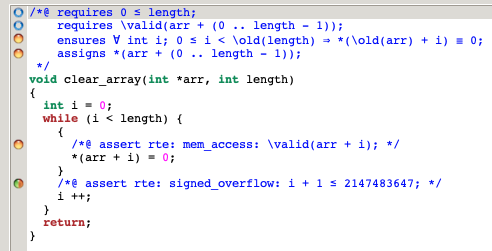
\includegraphics[width=0.6\textwidth]{images/frama_c_clear_array_post.png}
\end{center}

This is due to the fact that Frama-C does not know what to make of our for loop. Loops are difficult in deductive verification, since we usually do not a-priori know how many times we will execute them. If we knew, we would not need a loop in the first place, we could just copy the loop body the required amount of times (better leave that task to the compiler though!). Frama-C does not even know if the loop will actually ever terminate! So we have to supply a bit more information to help Frama-C in the proving procedure.

\section{Loop invariants} 

Certain things are true before we enter a loop, and they are still true at the end of every loop iteration. These kinds of properties are called \emph{loop invariants}. More precisely, a loop invariant is true whenever we check the looping condition. In our example function \textbf{clear\textunderscore array}, we have two invariants. One is about the iteration variable i, for which we know the lower and upper value boundry (zero and length respectively). The other is about the value of the array elements we have already set to zero. We can express this in the following way:

\ceditor{clear\textunderscore array.c}{code/loops/clear_array_invariants.c}

As you can see, we can annotate a loop inside a function with its own contract. Loop invariants are introduced with the \emph{loop invariant} keyword, and just like pre- and postconditions they are logical formulas. The two invariants we have introduced in the code shown above are hopefully self-explanatory. If we try and run Frama-C again on our changed contract, we unfortunately do not get a better result than before, so we still need to provide some more information. 

\section{Loop assignments}

Similar to how Frama-C could not automatically deduct which memory locations a function can access, it can also not reason about memory assignments inside a loop. We therefore have to manually provide a list of variables and locations that can change inside our loop body. This is done through the \emph{loop assigns} clause:

\ceditor{clear\textunderscore array.c}{code/loops/clear_array_assigns.c}

This pretty much follows the same syntax as the assigns clause for function contracts. Any variable that is visible in the function but is not listed in the loop assigns clause is considered to have the same value at the beginning and at the end of the loop execution. Lets see how Frama-C is doing with our new contract:

\begin{center}
    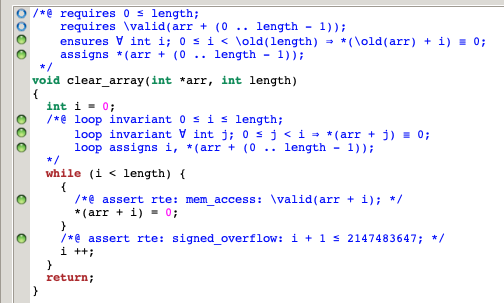
\includegraphics[width=0.6\textwidth]{images/frama_c_clear_array_assigns.png}
\end{center}

Fairly well! It could prove our postcondition and also verify that we do not change any memory locations outside of the boundries of the array. So let's try and see how it performs when used in another function: 

\ceditor{clear\textunderscore array.c}{code/loops/clear_array_main.c}

If we ask Frama-C to verify the above code, it will happily do so. However, we have actually not fully specified the intended behaviour of our function yet. 

\section{Loop variants}

There is an important notion in deductive program verification about the correctness of programs. What Frama-C tries to provide is a proof of partial correctness. This means, that it will try and prove our postconditions from our preconditions, \emph{assuming that the code we provide terminates}. We then call the proven program \emph{partially correct}.  If we can successfully prove its termination as well, then we speak of \emph{total correctness}. In our case, Frama-C actually succeeded in proving termination of the loop itself. This is not always the case. It is therefore good practice to define a \emph{loop variant}. A loop variant is an integer value that at each beginning of a loop iteration must be non-negative, and which must strictly decrease with each loop iteration. Providing such a loop variant allows Frama-C to prove termination of the loop itself. 

A complete contract for our \textbf{clear\textunderscore array} function looks like the following:

\ceditor{clear\textunderscore array.c}{code/loops/clear_array.c}

If Frama-C succeeds in proving the loop variant, we know that the loop will always terminate. 

\section{Exercises}

\subsection{Linrange function}

Implement and specify the following \textbf{linrange} function which takes as inputs an array, its length and a starting value, and assigns incrementing values to each array element starting with the start value:

\ceditor{linrange.c}{exercises/loops/linrange.c}

\subsection{Find minimum function}

Implement and specify the \textbf{find\textunderscore min} function, which takes an array of integers and the length of the array as input and returns the smallest element of the array: 

\ceditor{find\textunderscore min.c}{exercises/loops/find_min.c}

Depending on how you implement the function you might run into the problem that Frama-C is unable to prove part of your postcondition correct. This is most likely due to the fact that in your postcondition you made a statement regarding the index of the smallest element in the array. In a concise C implementation you do not have to actually save that index though. However, that means that Frama-C will have trouble using it in the deduction procedure. You have multiple options of how to mitigate that problem. You can either use a local variable that actually records the (current) position of the minimum element, or you can make use of a \textbf{ghost variable}. Ghost variables are variables that we need for the proof procedure, which are however not useful for the actual implementation of the algorithm. They have the advantage of not showing up in the final code and therefore saving space. You can read more on ghost variables in the ACSL manual \cite{baudin_acsl_nodate} in section 2.12. 
